%提案
\section{味覚変容システム}


%3.3 嗅覚
\subsection{嗅覚情報提示}
香りを嗅がせる方法として,図\ref{all}のような嗅覚情報提示装置を製作した.
香りを送るための仕組みを含んだボディやケースを3Dプリンタで作成している.
エアポンプから配送された風はチューブを通り,


\begin{figure}[t]
  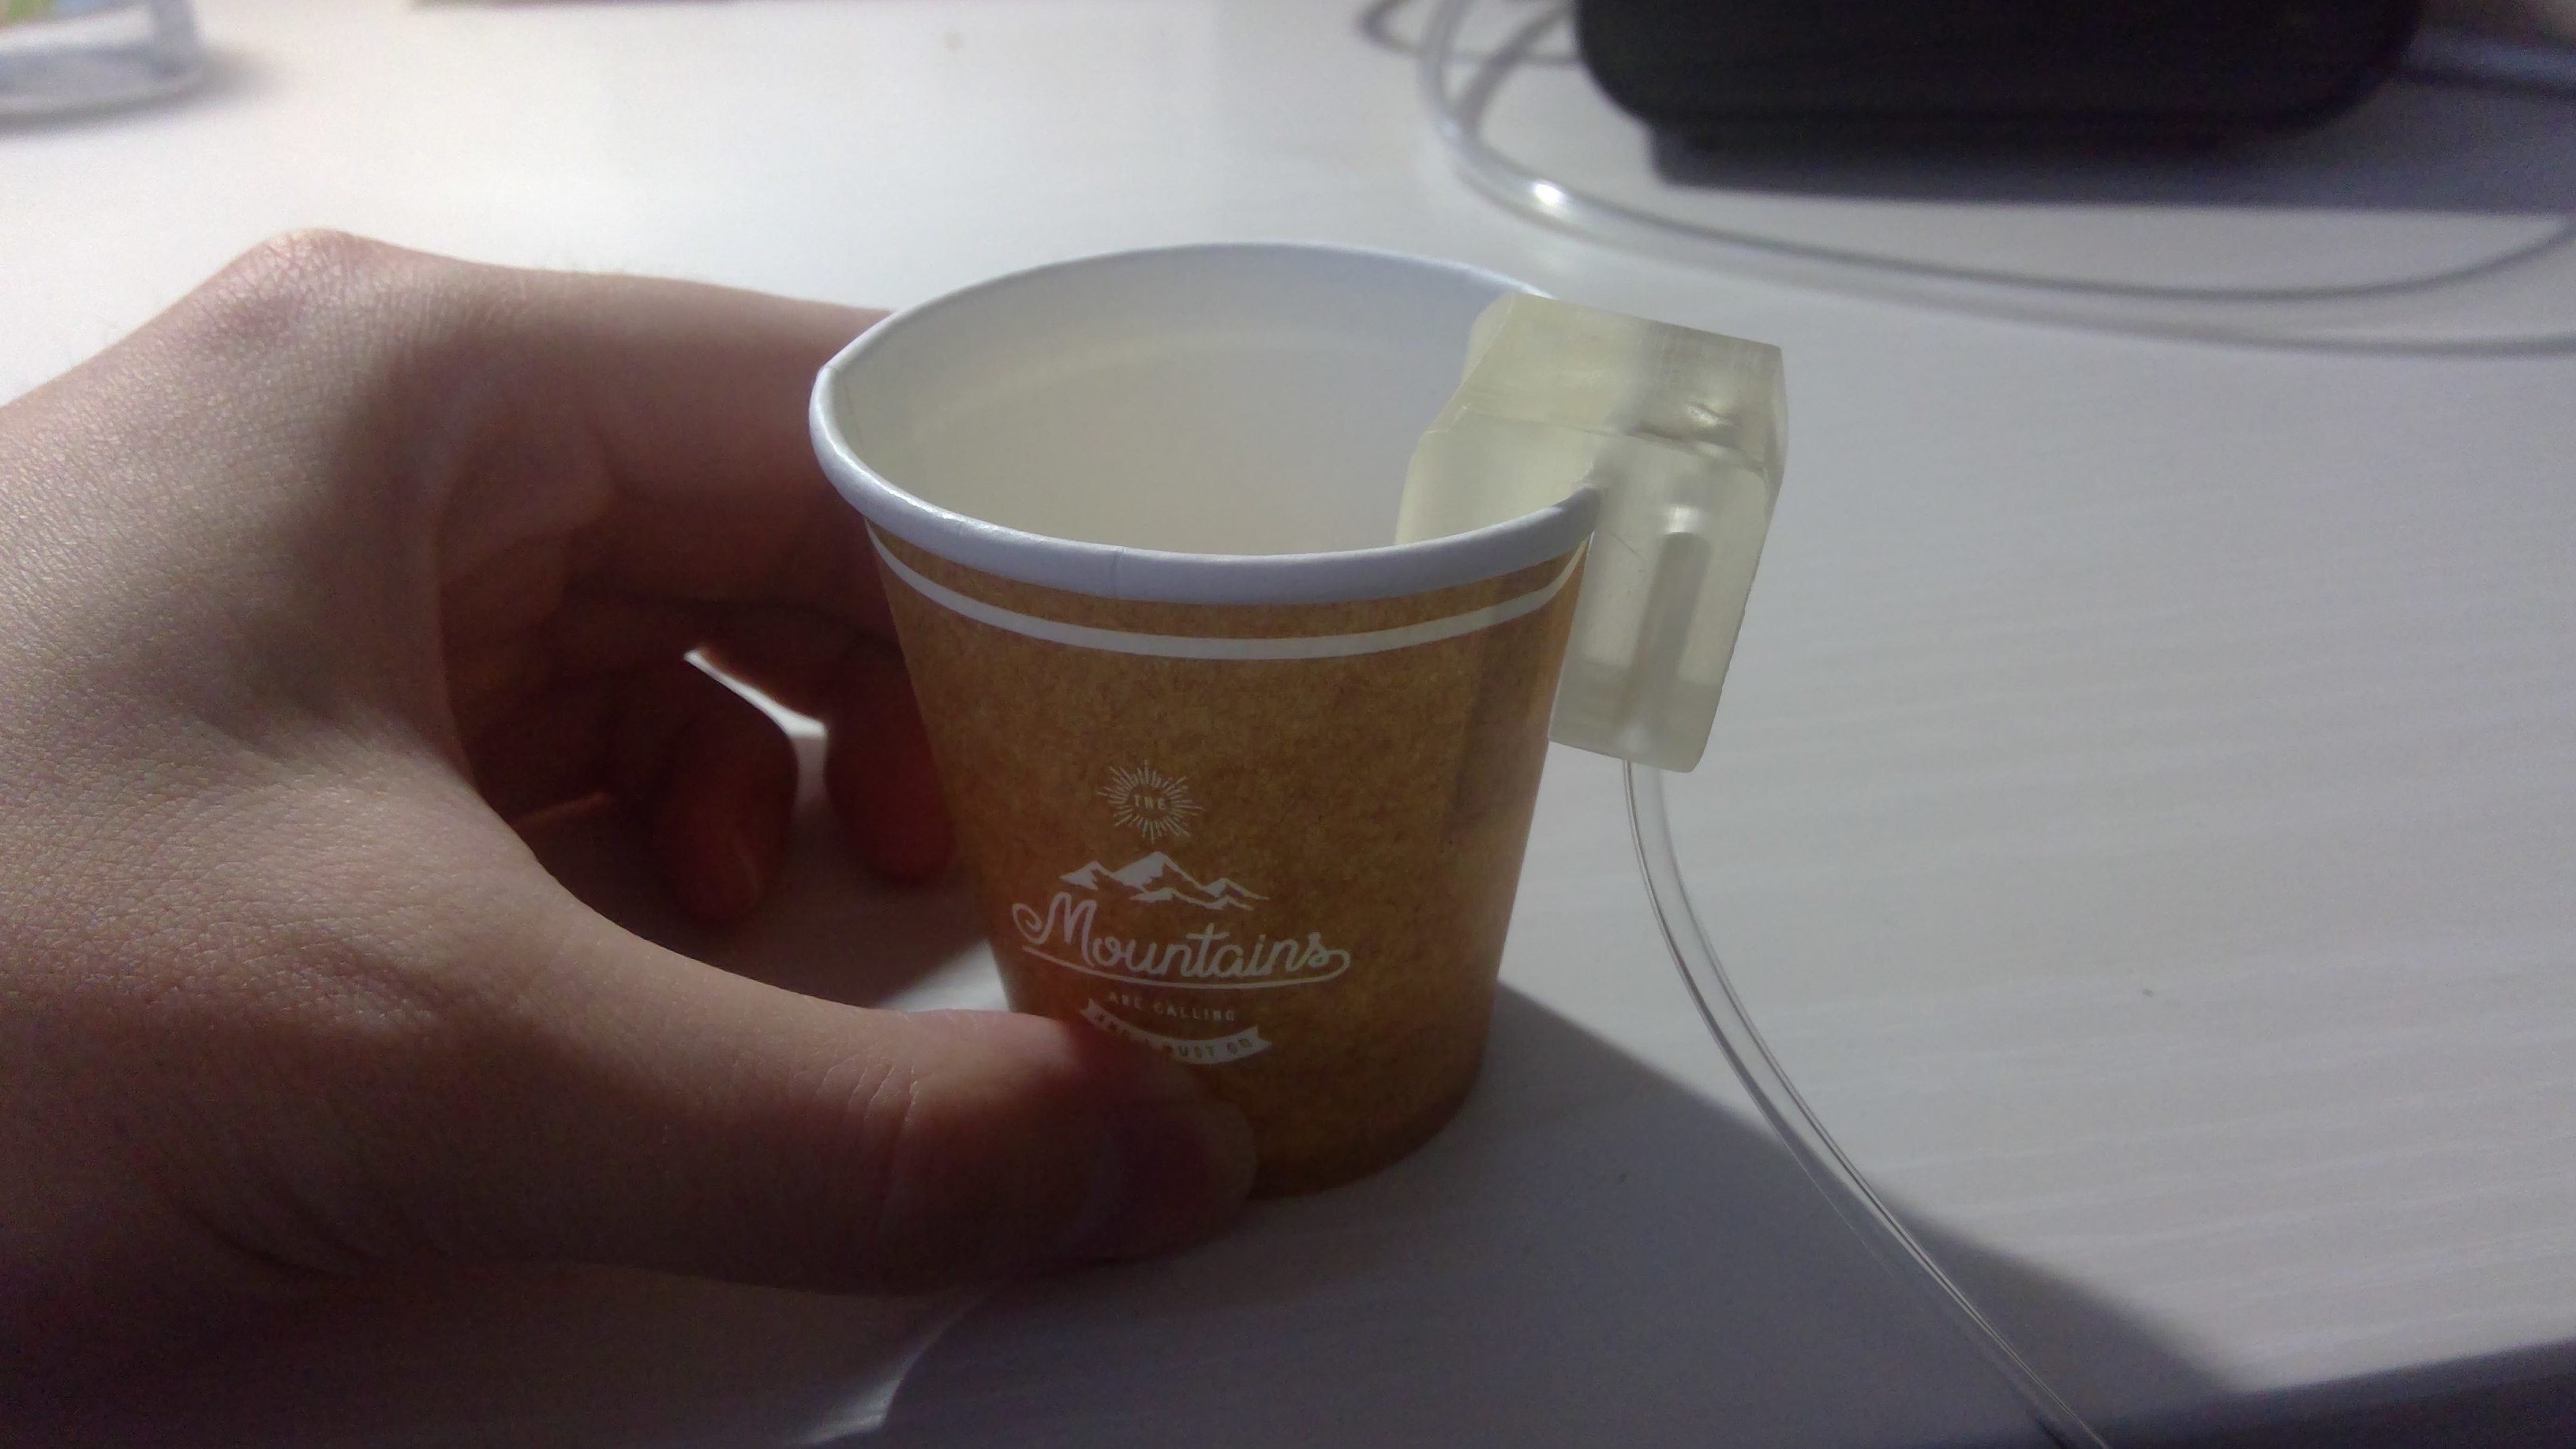
\includegraphics[width = 1.0\columnwidth]{figs/cup.jpg}
 %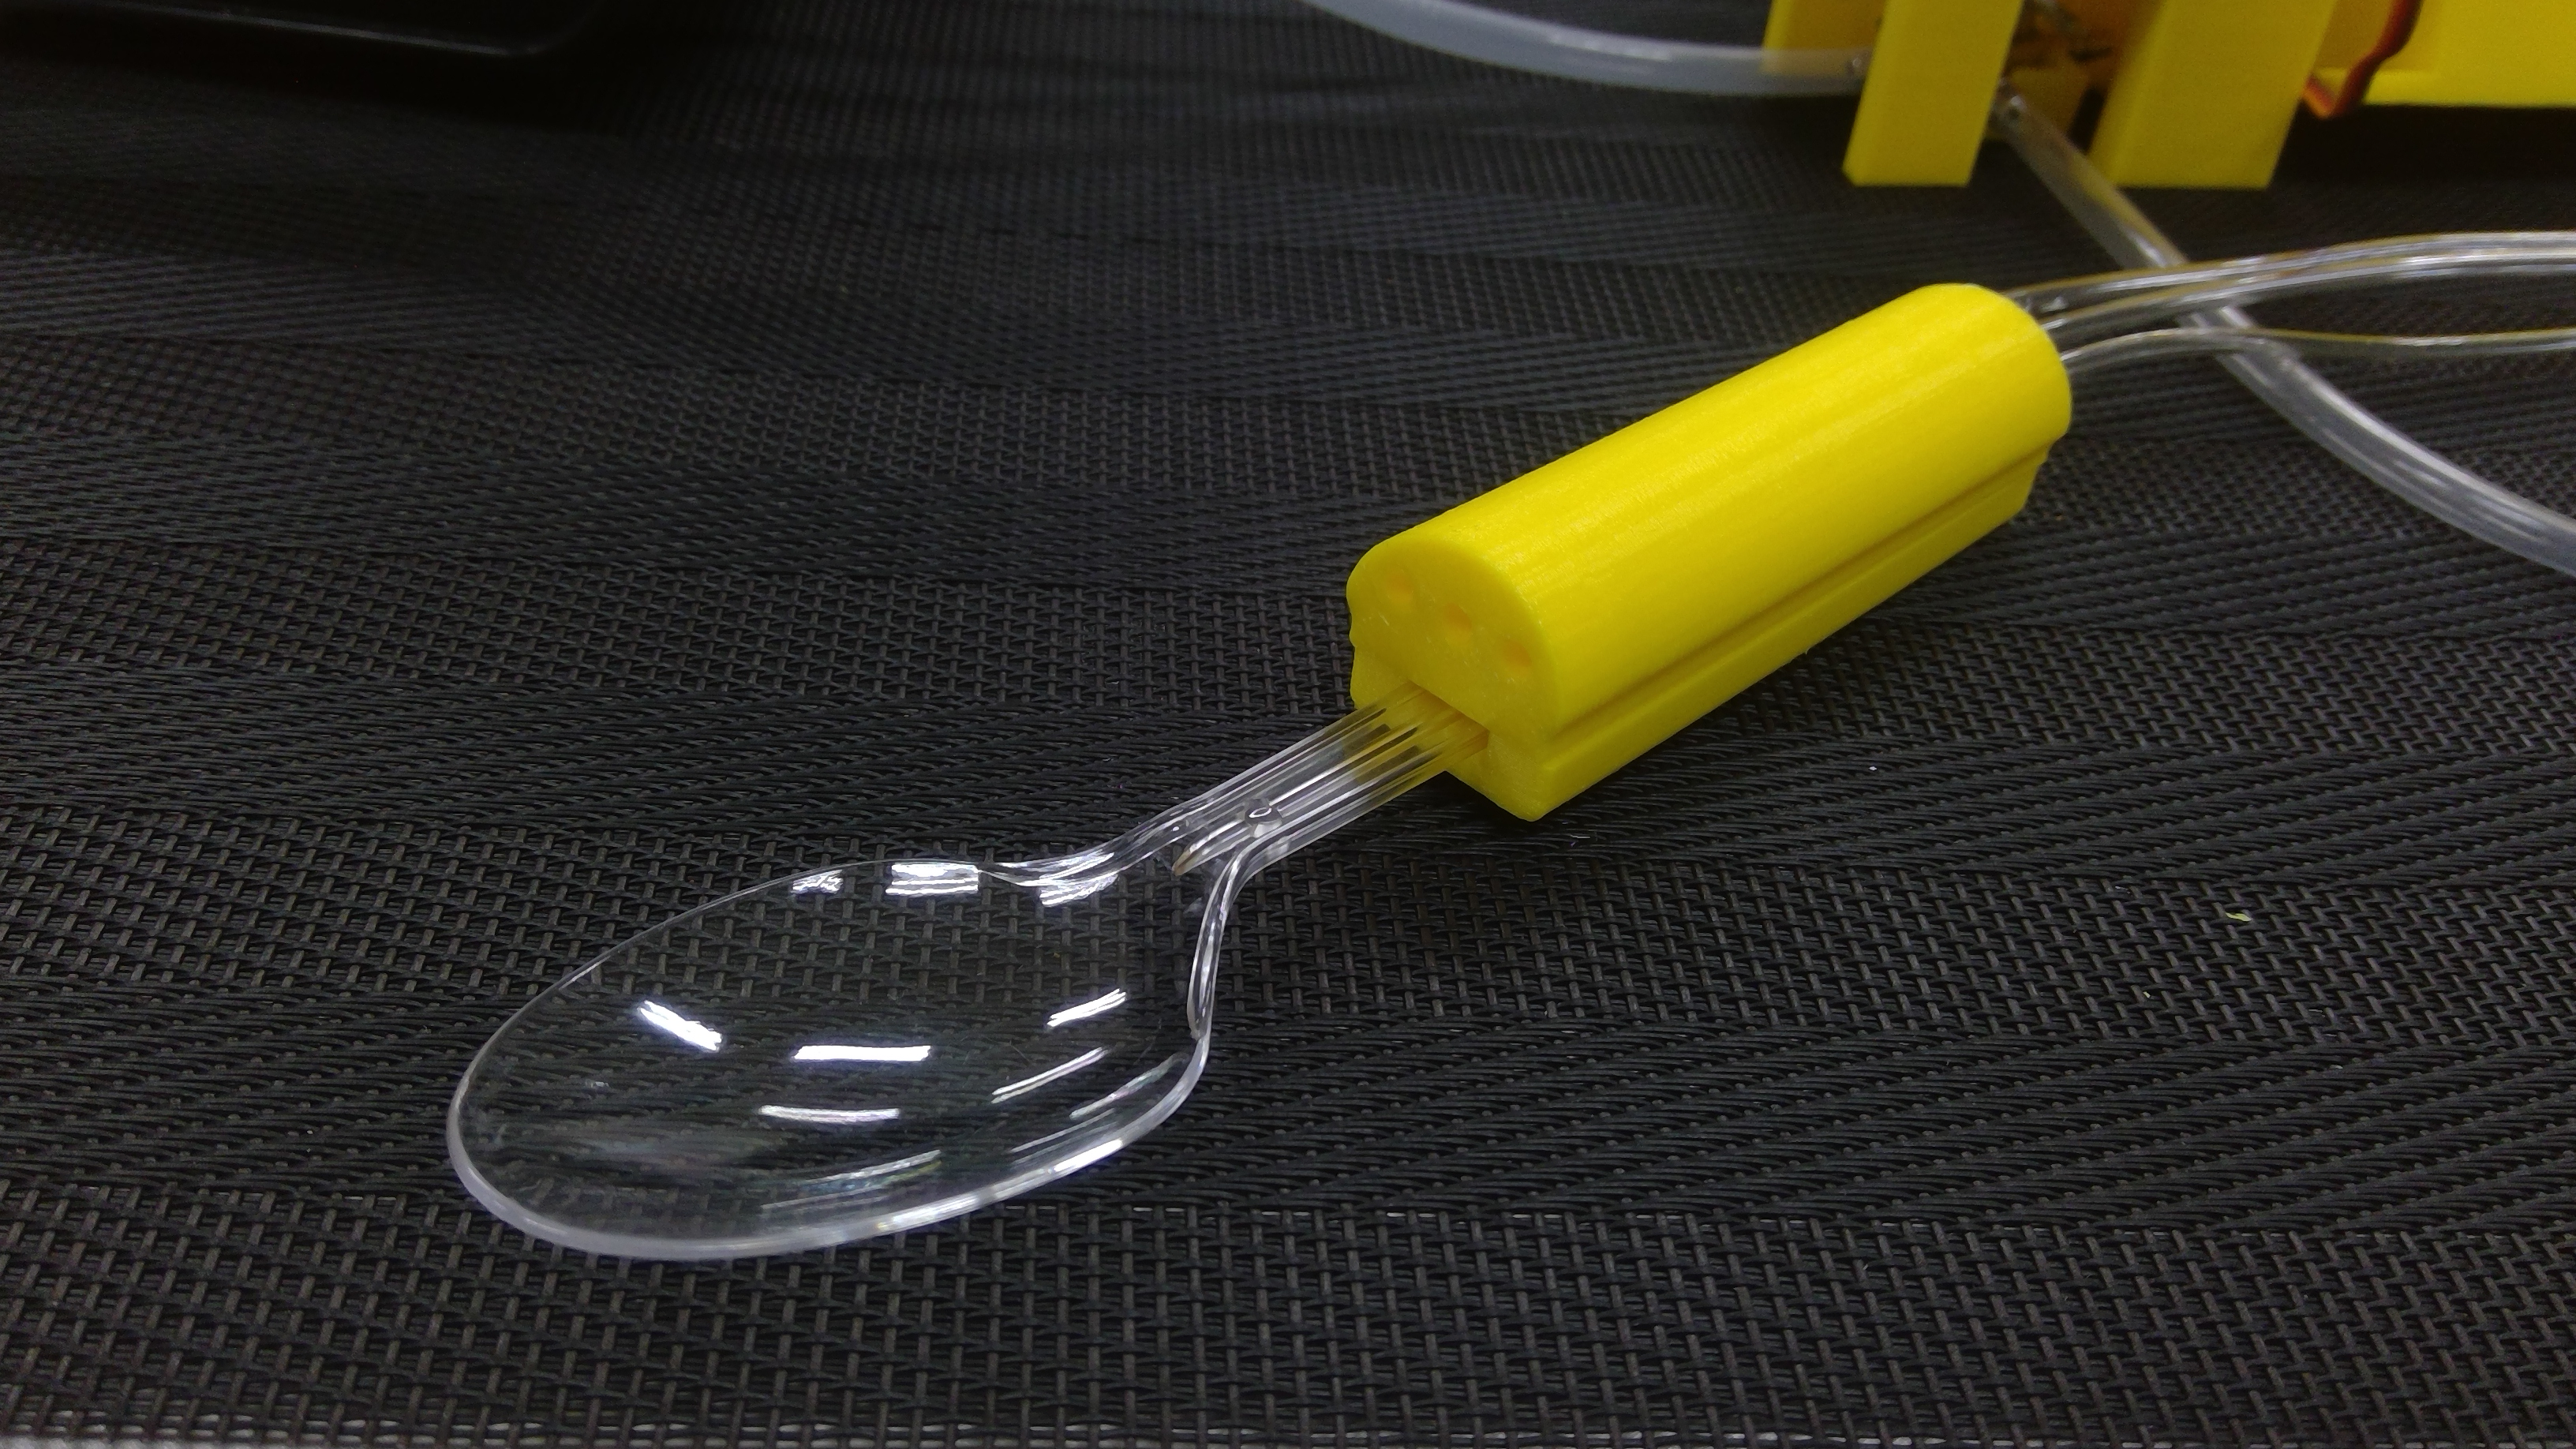
\includegraphics[width = 0.47\columnwidth]{figs/supunbody.jpg}
  \caption{嗅覚情報提示装置の全景}
  \ecaption{Panoramic view of olfactory information presentation device}
  \label{all}
\end{figure}

\begin{figure}[t]
  %\includegraphics[width = 0.47\columnwidth]{front2.jpg}
  %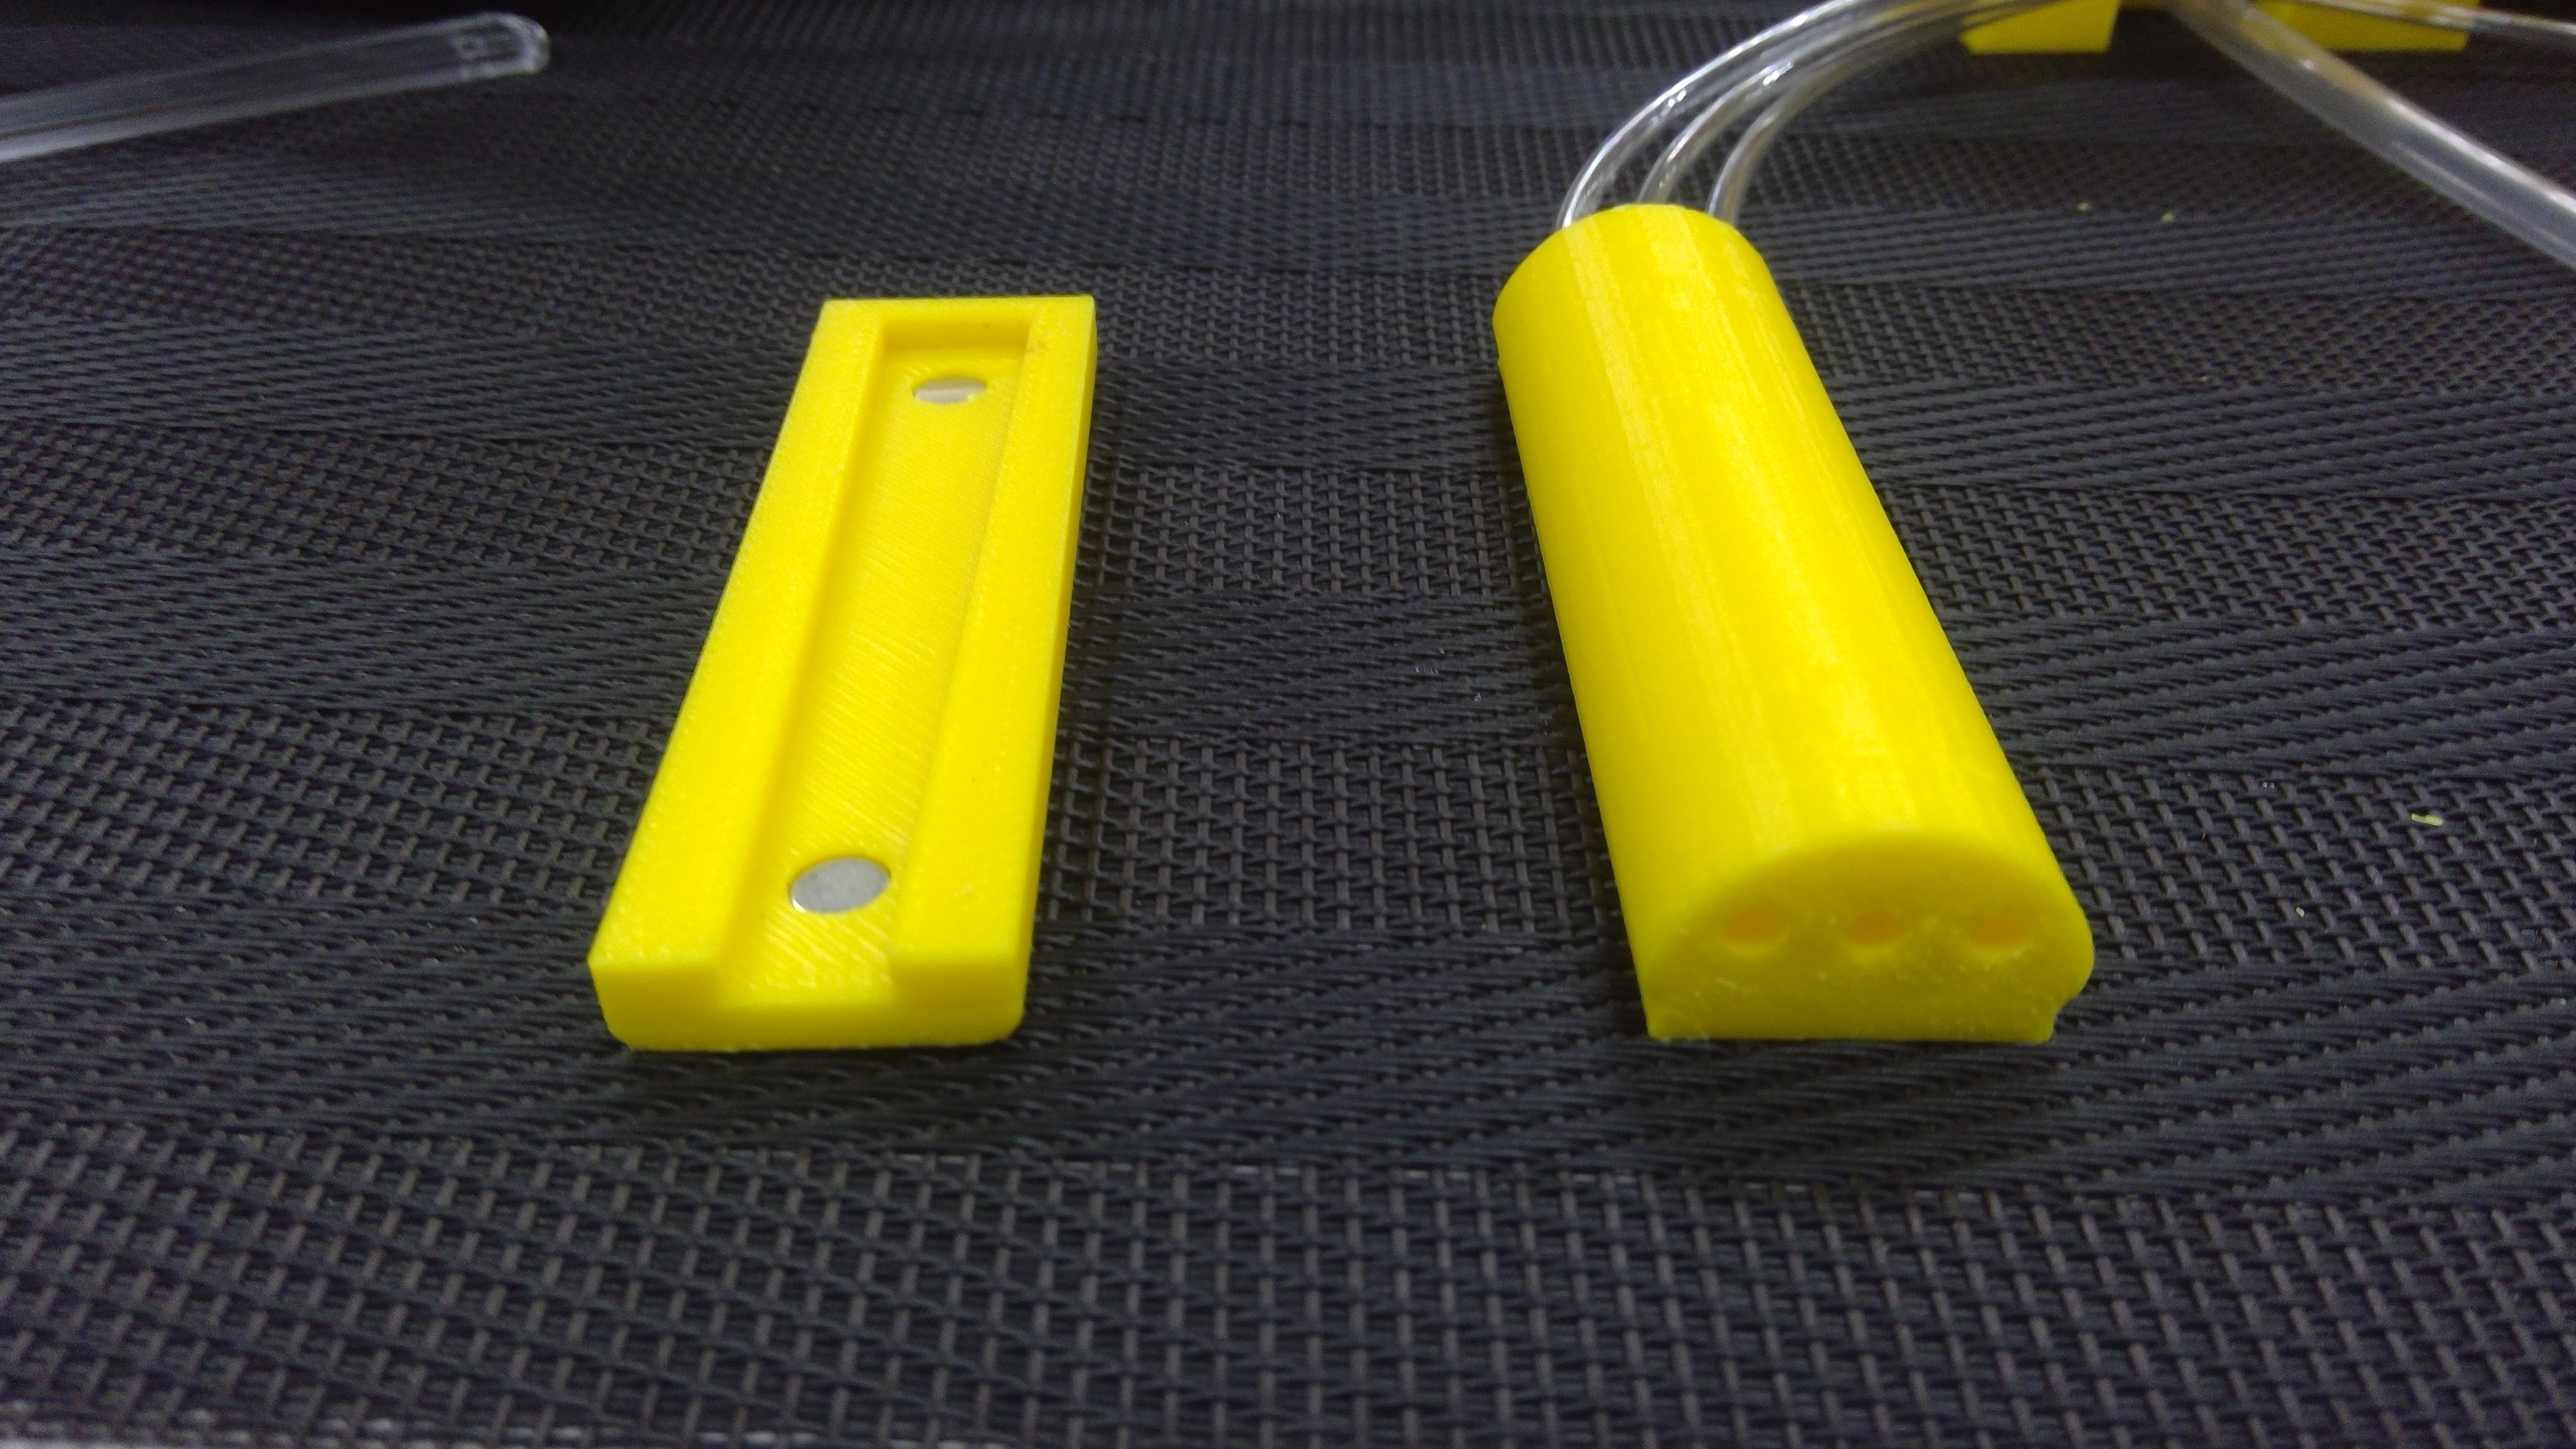
\includegraphics[width = 1.0\columnwidth]{supunpart.jpg}
  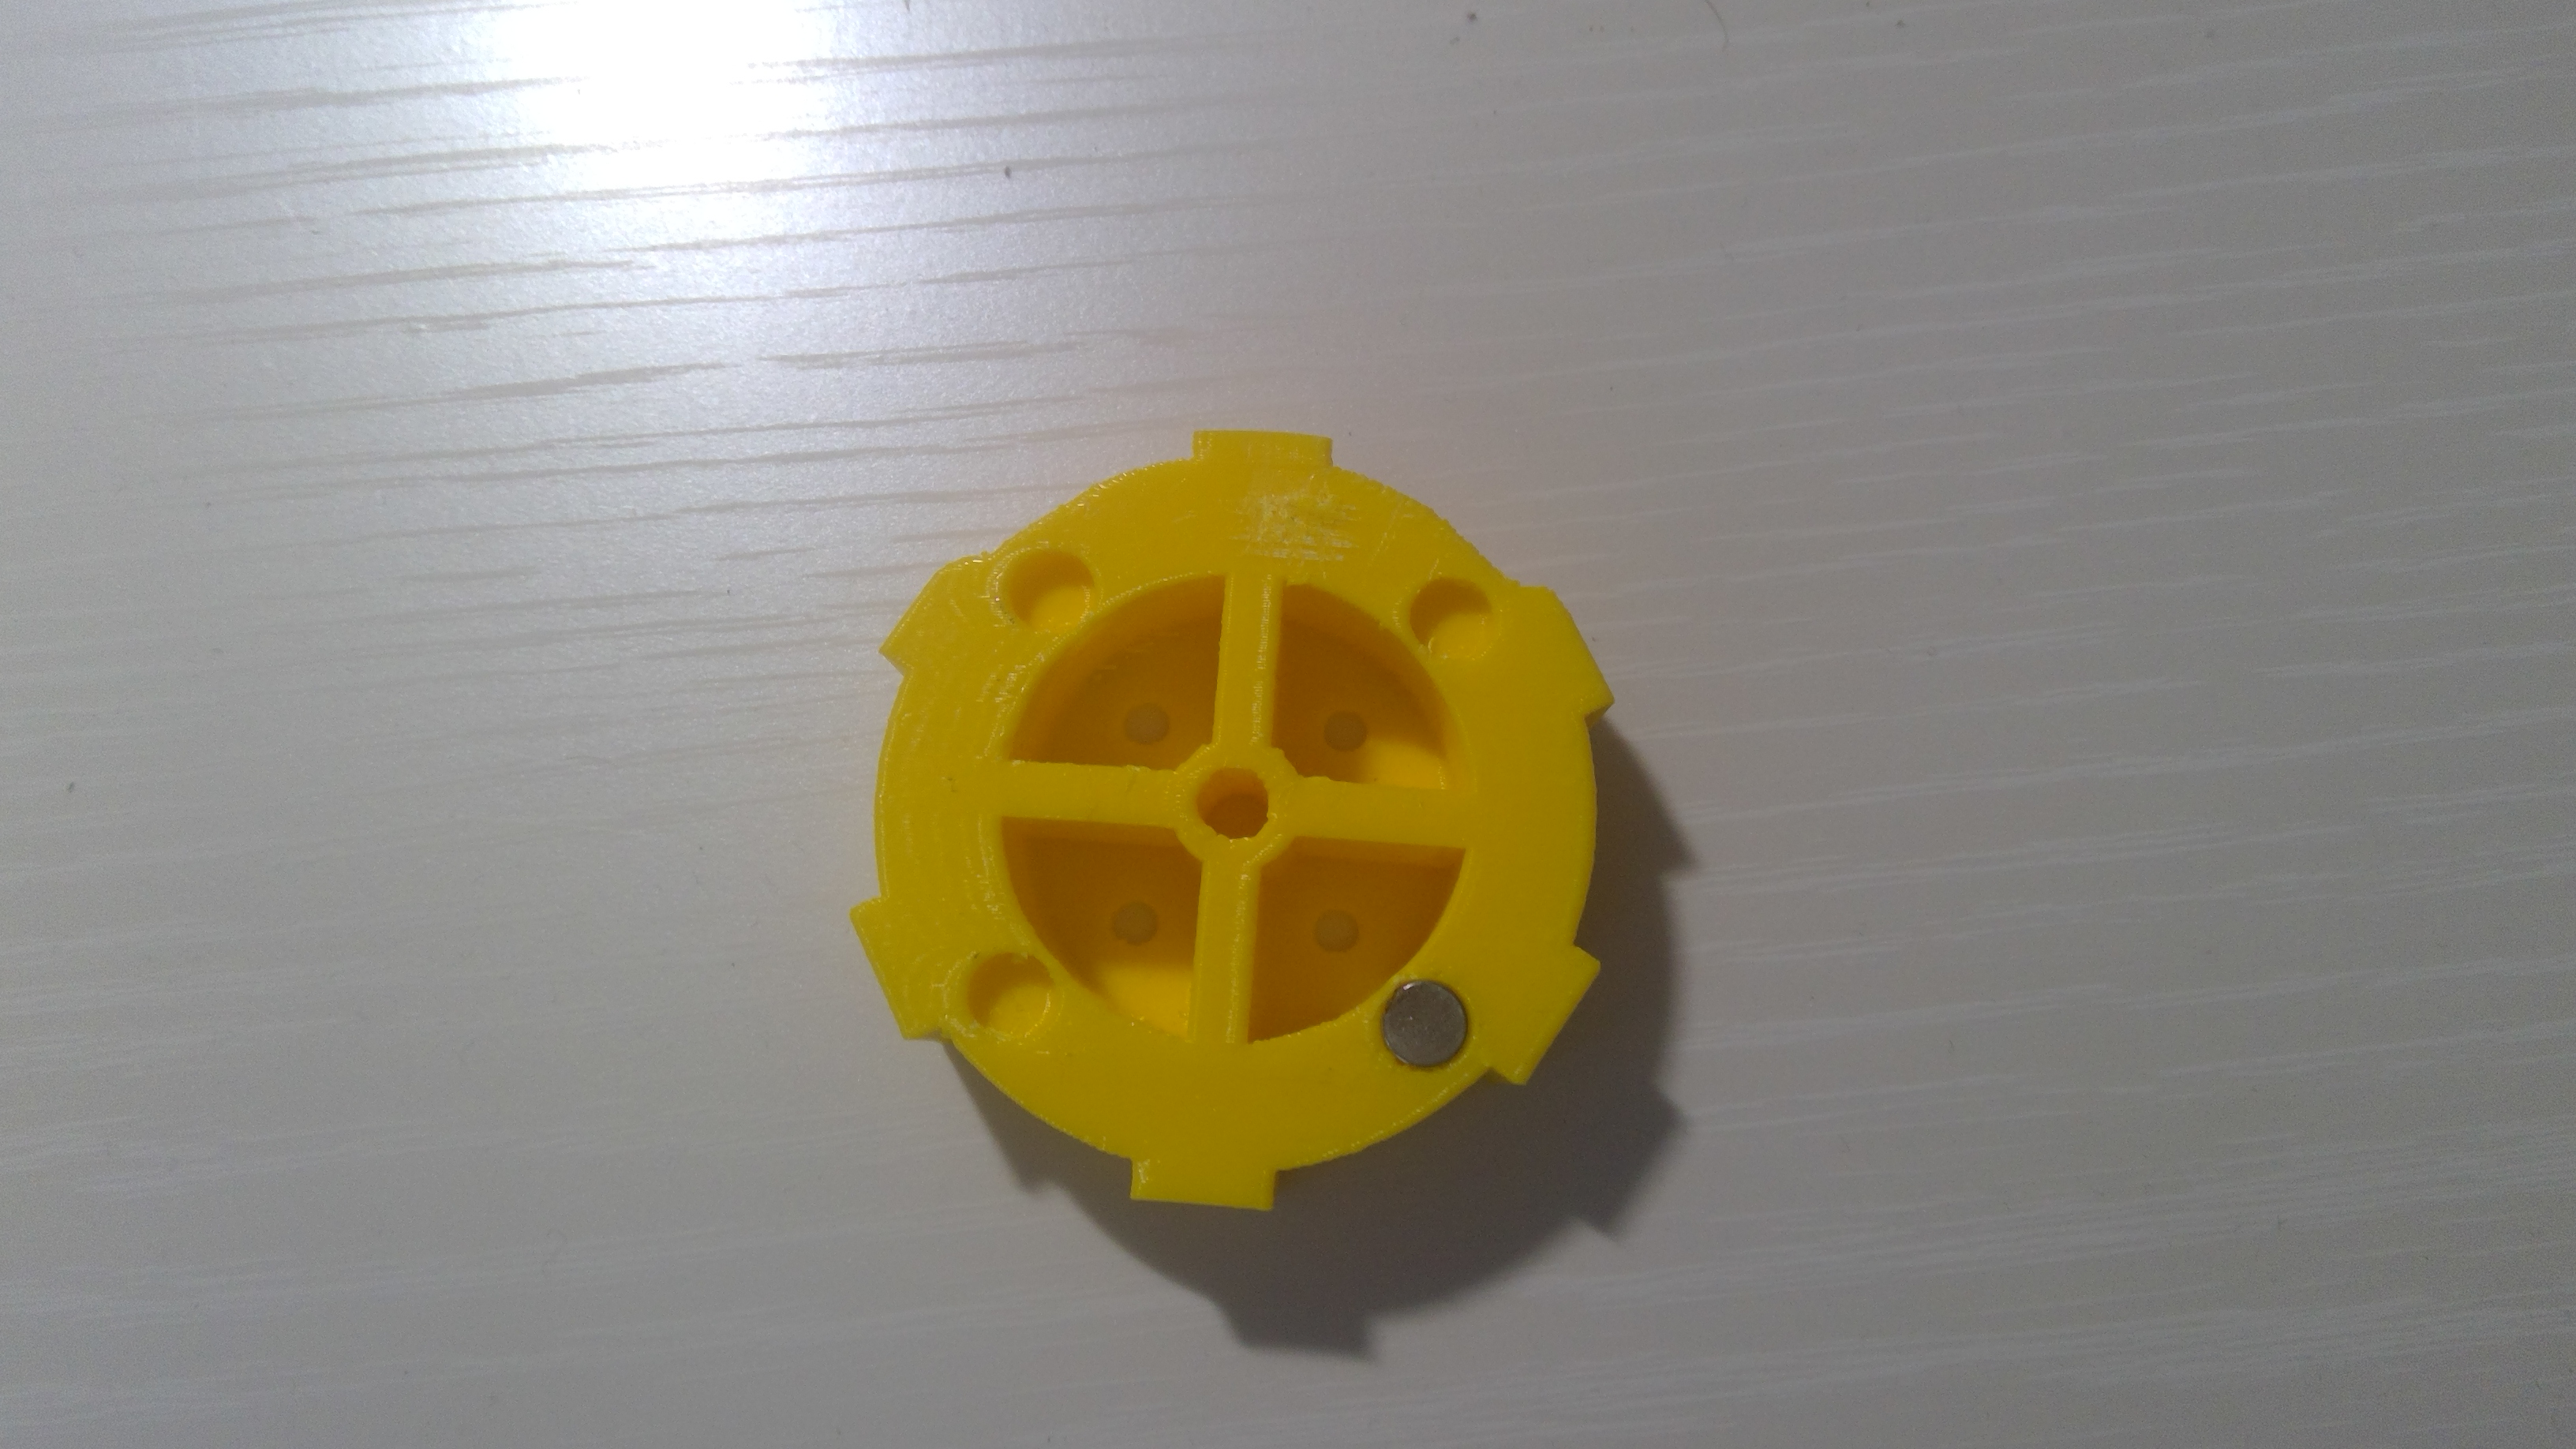
\includegraphics[width = 1.0\columnwidth]{figs/dial.jpg}
  \caption{香料切り替えデバイス}
  \ecaption{Spoon device}
  \label{device}
\end{figure}

使用する塩味スープを再現する香料の代わりとして,醤油・味噌の2種類の香りを外部刺激として使用する.
この二つは一般的に調味料としてしょっぱい味として認知されているものを選択した.




%本研究の目的は,嗅覚が与える影響を考慮し,それに視覚情報を加えることで,味覚に対しての認識を変化させることである.
%着色料を使用した色付けと食用の香料を含んだシロップで味わうかき氷においても視覚と嗅覚の違いで味に対する影響をもたらす.
%そのことから別の外部刺激で視覚と嗅覚にアプローチすることにより,通常のかき氷を同じような変化を再現することができるのではないかと仮説をたて検証した.
%そのために着色料を使用した色付けと食用の香料の代替品を用意し,嗅覚情報と視覚情報を提示するためのシステムを構築した.
%嗅覚面については香料の代わりとしてアロマオイル等の香りをファンを使用して鼻に伝達する.
%視覚面については着色料の代わりにLED光源を用いて色をつける.
%これら二つを組み合わせることで味覚変容を検討している.
